%% 
%% Copyright 2007-2024 Elsevier Ltd
%% 
%% This file is part of the 'Elsarticle Bundle'.
%% ---------------------------------------------
%% 
%% It may be distributed under the conditions of the LaTeX Project Public
%% License, either version 1.3 of this license or (at your option) any
%% later version.  The latest version of this license is in
%%    http://www.latex-project.org/lppl.txt
%% and version 1.3 or later is part of all distributions of LaTeX
%% version 1999/12/01 or later.
%% 
%% The list of all files belonging to the 'Elsarticle Bundle' is
%% given in the file `manifest.txt'.
%% 
%% Template article for Elsevier's document class `elsarticle'
%% with numbered style bibliographic references
%% SP 2008/03/01
%% $Id: elsarticle-template-num.tex 249 2024-04-06 10:51:24Z rishi $
%%
\documentclass[preprint,12pt]{elsarticle}
% \documentclass[final,5p,times,twocolumn]{elsarticle}

%% Custom packages
\usepackage[super]{nth}
\usepackage{amsfonts,amsthm,cancel,siunitx,calculator,calc,mathtools,empheq,latexsym}
\usepackage[version=4]{mhchem}
\usepackage[hyphens]{url} % allow line breaks in urls
\usepackage[breaklinks=true]{hyperref} % allow breakable links
\usepackage{booktabs,multicol,multirow,tabularx,array}
\usepackage[official]{eurosym}
\usepackage{subcaption}
\usepackage{placeins}
\usepackage{float}
\usepackage{tabularx}
\usepackage{booktabs}
\usepackage{enumitem}

\newcolumntype{R}[1]{>{\raggedleft\arraybackslash}p{#1}}

\graphicspath{
    {figures/}
  }
\DeclareGraphicsExtensions{.pdf,.jpeg,.jpg,.png}

%% Use the option review to obtain double line spacing
%% \documentclass[authoryear,preprint,review,12pt]{elsarticle}

%% Use the options 1p,twocolumn; 3p; 3p,twocolumn; 5p; or 5p,twocolumn
%% for a journal layout:
%% \documentclass[final,1p,times]{elsarticle}
%% \documentclass[final,1p,times,twocolumn]{elsarticle}
%% \documentclass[final,3p,times]{elsarticle}
%% \documentclass[final,3p,times,twocolumn]{elsarticle}
%% \documentclass[final,5p,times]{elsarticle}
%% \documentclass[final,5p,times,twocolumn]{elsarticle}

%% For including figures, graphicx.sty has been loaded in
%% elsarticle.cls. If you prefer to use the old commands
%% please give \usepackage{epsfig}

%% The amssymb package provides various useful mathematical symbols
\usepackage{amssymb}
%% The amsmath package provides various useful equation environments.
\usepackage{amsmath}
%% The amsthm package provides extended theorem environments
%% \usepackage{amsthm}

%% The lineno packages adds line numbers. Start line numbering with
%% \begin{linenumbers}, end it with \end{linenumbers}. Or switch it on
%% for the whole article with \linenumbers.
\usepackage{lineno}
\linenumbers

\journal{Nuclear Physics B}

\begin{document}

\begin{frontmatter}

%% Title, authors and addresses

%% use the tnoteref command within \title for footnotes;
%% use the tnotetext command for theassociated footnote;
%% use the fnref command within \author or \affiliation for footnotes;
%% use the fntext command for theassociated footnote;
%% use the corref command within \author for corresponding author footnotes;
%% use the cortext command for theassociated footnote;
%% use the ead command for the email address,
%% and the form \ead[url] for the home page:
%% \title{Title\tnoteref{label1}}
%% \tnotetext[label1]{}
%% \author{Name\corref{cor1}\fnref{label2}}
%% \ead{email address}
%% \ead[url]{home page}
%% \fntext[label2]{}
%% \cortext[cor1]{}
%% \affiliation{organization={},
%%             addressline={},
%%             city={},
%%             postcode={},
%%             state={},
%%             country={}}
%% \fntext[label3]{}

\title{The role of Projects of Common Interest in reaching Europe's energy policy targets}

%% use optional labels to link authors explicitly to addresses:
%% \author[label1,label2]{}
%% \affiliation[label1]{organization={},
%%             addressline={},
%%             city={},
%%             postcode={},
%%             state={},
%%             country={}}
%%
%% \affiliation[label2]{organization={},
%%             addressline={},
%%             city={},
%%             postcode={},
%%             state={},
%%             country={}}

\author[affi1]{Bobby Xiong\corref{cor1}} %% Author name
\author[affil1]{Iegor Riepin}
\author[affil1]{Tom Brown}

\cortext[cor1]{Corresponding author: \href{mailto:xiong@tu-berlin.de}{xiong@tu-berlin.de}}

%% Author affiliation
\affiliation[affi1]{organization={TU Berlin, Department of Digital Transformation in Energy Systems},
            % addressline={},
            city={Berlin},
            % postcode={},
            % state={},
            country={Germany}}

%% Abstract
\begin{abstract}
  The European Union (EU) aims to achieve climate-neutrality by 2050, with ambitious 2030 target, such as \SI{55}{\percent} greenhouse gas emissions reduction compared to 1990 levels, \SI{10}{Mt} p.a. of a domestic green \ce{H2} production, and \SI{50}{Mt} p.a. of \ce{CO2} injection capacity, which should be sequestered within the EU. 
  The European Commission selects so-called Projects of Common Interest (PCI) and Projects of Mutual Interest (PMI)---a large infrastructure projects for electricity, hydrogen and \ce{CO2} transport, and storage---that are of transnational importance as they link the energy systems of European countries.
  In this work, we evaluate the impact of PCI-PMI projects for the European energy system and EU energy policies. To achieve this, we investigate how delays in these projects could affect the EU's policy targets and examine potential conflicts between various policy objectives and the overarching greenhouse gas reduction goal. 
  \textbf{
  Our preliminary results for 2030 indicate that policy targets can be met even without PCI-PMI projects; however, these projects offer additional benefits: (i) \ce{H2} pipelines enhance the affordability and distribution of green \ce{H2}, thereby jumpstarting the hydrogen economy, and (ii) \ce{CO2} transport projects connect major industrial emissions to offshore sequestration sites in the North Sea.
  In our future work, we will analyse long-term pathway effects up to 2050, and incorporate hybrid interconnectors and \ce{CO2} shipping routes from the PCI-PMI list. 
  Overall, our findings highlight the critical interplay between cross-border cooperation, infrastructure investments, and policy targets in the European energy transition across all sectors.
  }
\end{abstract}

% %%Graphical abstract
% \begin{graphicalabstract}
% %\includegraphics{grabs}
% \end{graphicalabstract}

% %%Research highlights
% \begin{highlights}
% \item Research highlight 1
% \item Research highlight 2
% \end{highlights}

%% Keywords
\begin{keyword}
energy system modelling \sep energy policy \sep infrastructure \sep resilience \sep Europe \sep hydrogen \sep carbon  
%% keywords here, in the form: keyword \sep keyword

%% PACS codes here, in the form: \PACS code \sep code

%% MSC codes here, in the form: \MSC code \sep code
%% or \MSC[2008] code \sep code (2000 is the default)

\end{keyword}

\end{frontmatter}

%% Add \usepackage{lineno} before \begin{document} and uncomment 
%% following line to enable line numbers
%% \linenumbers

%% main text
%%

%% Use \section commands to start a section.
\section*{List of abbreviations}

\begin{itemize}[left=0pt, label={}, itemsep=0pt, parsep=0pt, topsep=0pt]
  \item \textbf{API} \enspace Application Programming Interface
  \item \textbf{EU} \enspace European Union
  \item \textbf{GHG} \enspace Greenhouse gas
  \item \textbf{PCI} \enspace Projects of Common Interest
  \item \textbf{PMI} \enspace Projects of Mutual Interest
  \item \textbf{REST} \enspace Representational State Transfer 
\end{itemize}

\section{Introduction}
\label{sec:introduction}
On the pathway to a climate-neutral Europe by 2050, the European Union (EU) has set ambitious targets for 2030. These targets include a reduction of \SI{55}{\percent} in greenhouse gas emissions compared to 1990 levels \cite{europeancommissionFit55Delivering2021}, \SI{10}{Mt} p.a. domestic green \ce{H2} production \cite{europeancommissionREPowerEUPlanCommunication2022}, and \SI{50}{Mt} p.a. of \ce{CO2} injection capacity with sequestration in within the EU \cite{europeanparliamentRegulationEU20242024}.

To support reaching these targets, the European Commission bi-annually identifies a list of Projects of Common Interest (PCI), which are key cross-border infrastructure projects that link the energy systems of the EU members, including transmission and storage projects for electricity, hydrogen and \ce{CO2} \cite{europeancommissionCommissionDelegatedRegulation2023}. 
The pool of project sutable for PCI status is based on projects submitted by transmission system operators, consortia, or third parties. Projects of Mutual Interest (PMI) further include cooperations with countries outside the EU, such as Norway or the United Kingdom. With a PCI-PMI status, project awardees receive strong political support and are, amongst others, eligible for financial support (e.g. through funding of the Connecting Europe Facility) and see accelerated permitting processes. On the other hand, project promoters are obliged to undergo comprehensive reporting and monitoring processes. 
In order for projects to be eligible for PCI-PMI status, their \textit{potential benefits need to outweigh their costs} \cite{europeancommissionCommissionDelegatedRegulation2023}. Given the political and lighthouse character, these projects are highly likely to be implemented. However, any large infrastructure project, including PCI-PMI projects, commonly face delays due to permitting, financing, procurement bottlenecks, etc. \cite{acerConsolidatedReportProgress2023}.

\subsection{Fuels, carriers, targets}
test

\subsection{Projects of Common/Mutual Interest}

This paper aims to evaluate the impact of PCI-PMI projects on the European energy system and EU energy policies. We focus on the following key research questions:

\begin{enumerate} 
  \item What is the impact of delay in PCI-PMI projects' realisation on the EU's policy targets for 2030?
  \item What are the costs associated with adhering to the EU policy targets, even if PCI-PMI projects are delayed? 
  \item Do the green hydrogen production and carbon sequestration targets conflict with the cost-effective achievement of the greenhouse gas emission reduction goals? 
\end{enumerate}

\newpage
\section{Literature review}
\label{sec:literature_review}

\newpage
\section{Methodology}
\label{sec:methodology}

We use the open-source, sector-coupled energy system model PyPSA-Eur \cite{neumannPotentialRoleHydrogen2023,frysztackiComparisonClusteringMethods2022,glaumOffshorePowerHydrogen2024,horschPyPSAEurOpenOptimisation2018} to optimise investment and dispatch decisions for generation, storage, transmission energy infrastructure, as well as conversion technologies in the European energy system.



A space of model endogenous decisions includes expansion of renewable energy sources and dispatchable power plants, electricity storage technologies, power-to-X conversion capacities, transmission infrastructure for power, hydrogen, and \ce{CO2}, heating technologies, as well as technology stacks for gray, blue or green hydrogen production, among others. 
The model also considers various energy carriers like electricity, heat, hydrogen, \ce{CO2}, methane, methanol, liquid hydrocarbons, and biomass, as well as a broad range of conversion technologies.
The model is spatially and temporally highly resolved and covers the entire European continent, including stocks of existing power plants \cite{gotzensPerformingEnergyModelling2019}, renewable potentials, and availability time series \cite{hofmannAtliteLightweightPython2021}. It covers today's high-voltage transmission grid (AC \SI{220}{kV} to \SI{750}{kV} and DC \SI{150}{kV} upwards) \cite{xiongModellingHighVoltageGrid2024}.

\subsection{Feature implementation}
\label{sec:feature_implementation}

By accessing the REST API of the PCI-PMI Transparency Platform \cite{europeancommissionPCIPMITransparencyPlatform2024} and associated public project sheets provided by the European Commission, we implement the PCI-PMI projects into the PyPSA-Eur model to assess their impact in the power, heat, transport, industry, feedstock, and agriculture sector. Note that we use standardised costs for all PCI-PMI projects \cite{zeyenPyPSATechnologydataV0922024} for two reasons: (i) Cost data provided by project promoters can be incomplete and may not include the same cost components, and (ii) to ensure comparability as well as level-playing field between all potential projects, including both PCI-PMI and model-endogenous investments.
Our implementation can adapt to the needs and configuration of the model, including selected technologies, geographical and temporal resolution, as well as the level of sector-coupling. An overview of the implemented PCI-PMI projects is shown in Figure \ref{fig:regional_scope_map}.

\begin{figure}[htbp]
  \centering
  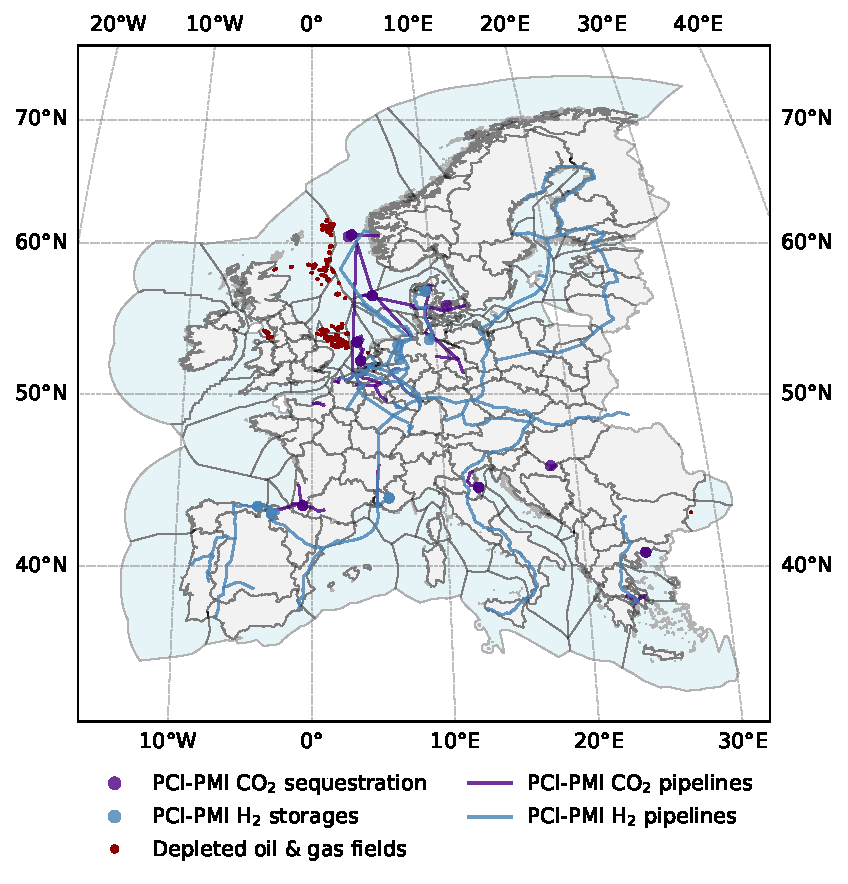
\includegraphics[width=1\linewidth]{regional_scope_map}
  \caption{Map of the regional scope including clustered onshore (grey) and offshore regions (blue), as well as PCI-PMI \ce{CO2} and \ce{H2} pipelines, storage and sequestration sites. Depleted offshore oil and gas fields (red) provide additional \ce{CO2} sequestration potential. Own illustration based on \cite{hofmannH2CO2Network2025} and data from the European Commission \cite{europeancommissionPCIPMITransparencyPlatform2024}.}
  \label{fig:regional_scope_map}
\end{figure}

\subsection{Scenario setup}
\label{sec:scenario_setup}

As of the date of submission, we model three key scenarios for the target year 2030 which will set the base year for pathways towards 2050: a \textit{Base} scenario in which policy targets are achieved and all projects are commissioned on time as well as two PCI-PMI delay scenarios \textit{A} and \textit{B}. Table \ref{tab:scenarios} gives an overview of the scenarios' key assumptions and their differences. Depending on the scenario, we formulate and activate additional constraints to ensure the fulfilment of the EU policy targets.

\begin{table*}[htbp]
  \centering
  \caption{Scenario matrix setup. Own illustration.}
  \label{tab:scenarios}
  \scriptsize
  \begin{tabularx}{\textwidth}{R{4.1cm}>{\centering\arraybackslash}X>{\centering\arraybackslash}X>{\centering\arraybackslash}X}
    \toprule
    \textbf{Short-term} & \textbf{Reduced targets} & \textbf{Delayed pipelines} & \textbf{No pipelines} \\
    \midrule
    \textbf{Long-term scenarios} & & & \\
    i. No pipelines & $\blacksquare$ & -- & -- \\
    ii. PCI-PMI projects & $\blacksquare$ & $\blacksquare$ & $\blacksquare$ \\
    iii. (ii.) + national expansion & $\blacksquare$ & $\blacksquare$ & $\blacksquare$\\
    iv. (iii.) + internat. expansion & $\blacksquare$ & $\blacksquare$ & $\blacksquare$ \\
    v. Greenfield & $\blacksquare$ & $\blacksquare$ & $\blacksquare$ \\
    \midrule
    \textbf{Targets} & & & \\
    GHG emission reduction &  $\blacksquare$ &  $\blacksquare$ &  $\blacksquare$ \\
    \ce{CO2} sequestration &  -- &  $\blacksquare$ &  $\blacksquare$ \\
    Green \ce{H2} production &  -- &  $\blacksquare$ &  $\blacksquare$ \\
    \ce{H2} electrolysers &  -- &  $\blacksquare$ &  $\blacksquare$ \\
    \midrule
    \textbf{\ce{CO2} + \ce{H2} infrastructure} & & & \\
    \ce{CO2} sequestration sites & $\blacksquare$ &  $\blacksquare$ &  $\blacksquare$ \\
    \ce{CO2} pipelines to offs. seq. site & $\blacksquare$ &  $\blacksquare$ &  $\blacksquare$ \\
    \ce{CO2} onshore pipelines & $\blacksquare$ &  $\square$ &  -- \\
    \ce{H2} pipelines & $\blacksquare$ &  $\square$ &  -- \\
    \midrule
    \textbf{Model configuration} & & & \\
    Planning horizons &  \multicolumn{3}{c}{Myopic: [2030, 2040, 2050] } \\
    Electricity grid & \multicolumn{3}{c}{OSM, TYNDP, NEP, PCI-PMI} \\

    \bottomrule
  \end{tabularx}
  \caption*{\scriptsize $\blacksquare$ active \quad $\square$ delayed by one period \quad -- inactive}
\end{table*}


\begin{table*}[htbp]
  \centering
  \caption{Pathway for implemented targets. Own illustration.}
  \label{tab:targets}
  \scriptsize
  \begin{tabularx}{\textwidth}{R{4.1cm}>{\centering\arraybackslash}X>{\centering\arraybackslash}X>{\centering\arraybackslash}X}
    \toprule
    \textbf{Planning horizon} & \textbf{2030} & \textbf{2040} & \textbf{2050} \\
    \midrule
    \textbf{Targets} & & & \\
    GHG emission reduction &  \SI{-55}{\percent} & \SI{-90}{\percent} & \SI{-100}{\percent} \\
    \ce{CO2} sequestration & \SI{50}{Mtpa} & \SI{150}{Mtpa} & \SI{250}{Mtpa} \\
    Green \ce{H2} production & \SI{10}{Mtpa} & \SI{27.5}{Mtpa} & \SI{45}{Mtpa} \\
    \ce{H2} electrolysers & \SI{40}{GW} &  \SI{110}{GW} &  \SI{180}{GW} \\
    \bottomrule
  \end{tabularx}
\end{table*}

\newpage
\section{Results and discussion}
\label{sec:results_and_discussion}

\paragraph{Base scenario} Figure \ref{fig:balance_maps_base} shows the regional distribution of the \ce{H2} and \ce{CO2} value chain in the Base scenario. Note that for the specific year of 2030, a disconnect in \ce{H2} infrastructure between central and southeastern Europe can be observed, due to the delay in commissioning of the project connecting the two networks. Within the two interconnected regions, almost homogenous average marginal prices for \ce{H2} can be observed. Note that Figure \ref{fig:balance_map_h2_base} shows the cost of all \ce{H2} produced, weighted by the respective regional demand at a certain point in time. \ce{CO2} prices are higher in demand regions for industry processes and methanolisation located in northwestern Europe --- primarily Norway and the United Kingdom (Figure \ref{fig:balance_map_co2_base}). Negative \ce{CO2} prices in souhtheastern Europe indicate a lack of demand and missing economic value.
Utilisation of \ce{H2} pipelines vary strongly across the PCI-PMI projects. In most of the times, pipelines serve the purpose of transporting \ce{H2} in a single direction only, i.e. from high renewable potential regions to \ce{H2} consumption sites, where it serves as a precursor for methanolisation or direct use in industry and shipping (see Figure \ref{fig:balance_map_h2_base}). Prominent PCI-PMI projects with particularly high full-load hours include P9.9.2 \textit{Hydrogen Interconnector Denmark-Germany} (\SI{6937}{h}) and P11.2  \textit{Nordic-Baltic Hydrogen Corridor} (\SI{2295}{h}), followed by projects connecting major steel-industrial and chemical sites of Germany (southwest) with Belgium (P9.4 \textit{H2ercules West}, \SI{1634}{h}), the Netherlands (P9.6 \textit{Netherlands National Hydrogen Backbone}, \SI{1967}{h} and P9.7.3 \textit{Delta Rhine Corridor H2}, \SI{1510}{h}), and France (P9.2.2 \textit{MosaHYyc}, \SI{4662}{h}). PCI project P13.8 \textit{EU2NSEA} connects \ce{CO2} from process emissions in Germany, Belgium and the Netherlands to major geological sequestration sinks close to the Norwegian shore \textit{Smeaheia} and \textit{Luna} with an annual injection potential of \SI{20}{Mt} p.a. and {5}{Mt} p.a., respectively. 

\begin{figure*}[htbp]
  \centering
  \begin{subfigure}[t]{0.47\textwidth} % [t] aligns at the top
      \vspace{0pt}
      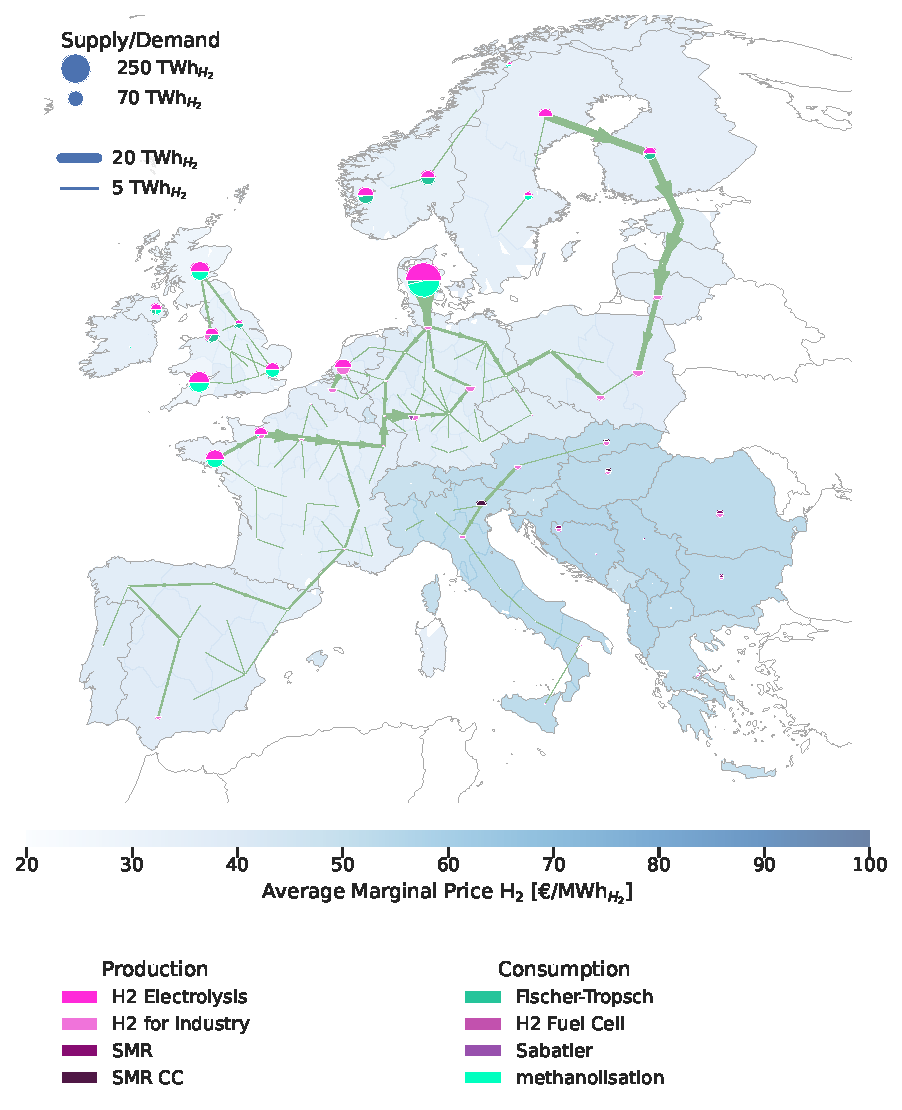
\includegraphics[width=0.9\textwidth]{balance_map_h2_base} % Replace with your image
      \vspace{0.3cm}
      \caption{\ce{H2} regional balances and flows (all \ce{H2} produced).}
      \label{fig:balance_map_h2_base}
  \end{subfigure}
  \hfill
  \begin{subfigure}[t]{0.47\textwidth} % [t] aligns at the top
      \vspace{0pt}
      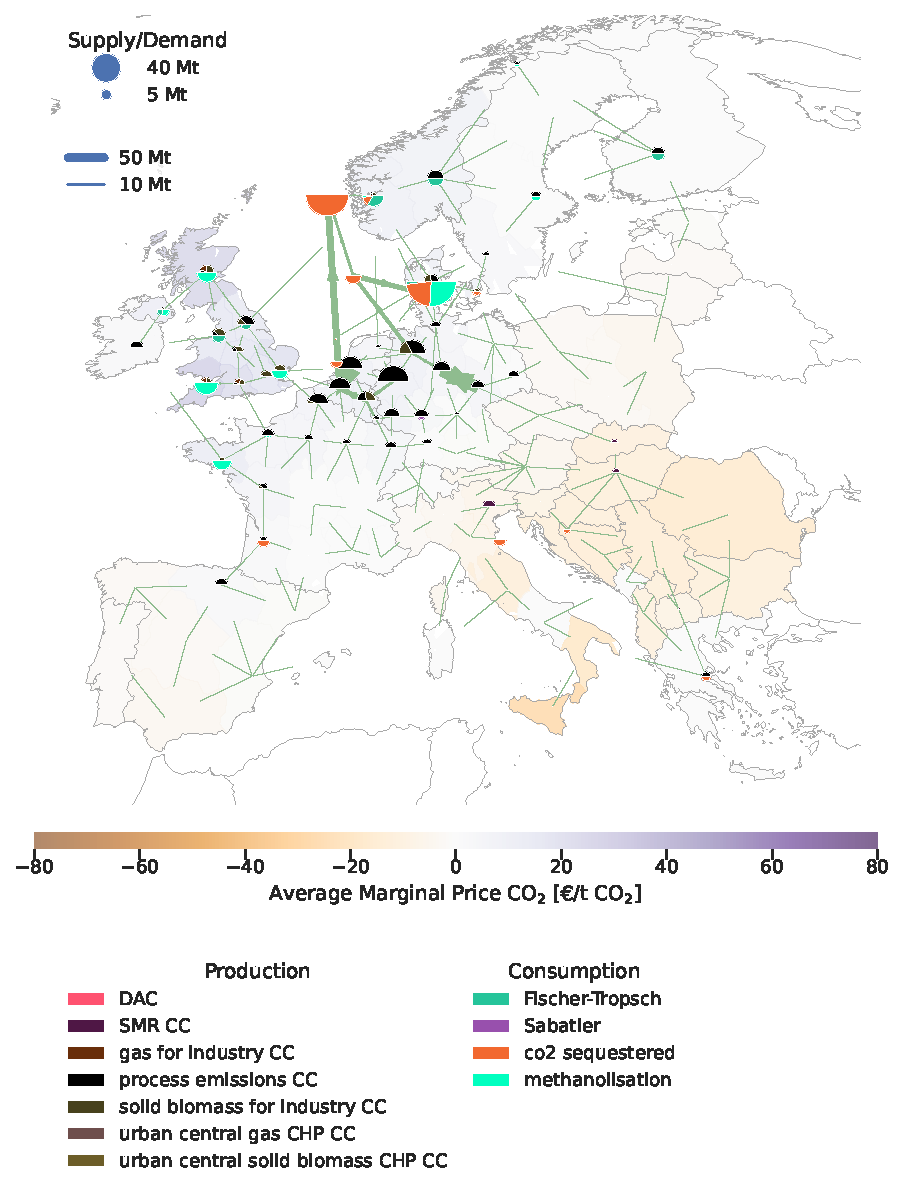
\includegraphics[width=0.9\textwidth]{balance_map_co2_base} % Replace with your image
      \caption{\ce{CO2} regional balances and flows.}
      \label{fig:balance_map_co2_base}
  \end{subfigure}
  \caption{Results \textit{Base} scenario --- Regional distribution of \ce{H2} and \ce{CO2} production, utilisation, storage, and transport in the Base scenario. Own illustration.}
  \label{fig:balance_maps_base}
\end{figure*}

\paragraph{Scenario A compared to Base} PCI-PMI infrastructure account for a total of around 30 bn. \euro{} p.a. in additional total system costs, indicating that for the target year 2030, the projects are not cost-optimal. With a delay of PCI-PMI projects in scenario \textit{A}, Europe's policy targets can still be achieved at significantly lower cost. However, this comes at the expense of a less interconnected energy system, which may lead to higher costs in the long run. Further, \ce{H2} prices vary more strongly across regions, seeing higher costs in southeastern Europe due to industrial demand and lower renewable potentials (Figure \ref{fig:balance_map_h2_scenario_a}). We make similar observations for \ce{CO2} --- a lack of pipeline infrastructure increases spread of \ce{CO2} prices, seeing higher values for \ce{CO2} in regions with high demand (e.g. for industrial processes or methanolisation). 

\paragraph{Scenario B compared to Base}
By omitting a green \ce{H2} target, almost no electrolysers are installed. Around \SI{8}{Mt} are still produced to cover industrial \ce{H2} and methanol (primarily shipping) demand (Figures \ref{fig:h2_balance} and \ref{fig:co2_balance}). However, this demand is met by decentral steam methane reforming instead of electrolysers (Figure \ref{fig:h2_balance}). 
Without specifying a \ce{CO2} sequestration target, the system still collects around \SI{21}{Mt} of \ce{CO2} p.a. primarily from process emissions in the industry sector and sequesters it in carbon sinks near industrial sites where a sequestration potential is identified (see Figure \ref{fig:regional_scope_map}) \cite{hofmannH2CO2Network2024}. This carbon sequestration is incentivised by the emission constraint for 2030. As no pipeline infrastructure is built in these scenarios, the chosen locations differ in the delay scenarios --- this can be observed for regions near the coast, such as the United Kingdom and Norway (see Figure \ref{fig:regional_scope_map}). Given the lack of infrastructure, both the average cost for \ce{H2} and \ce{CO2} are higher in scenario \textit{B} compared to the Base scenario (Figures \ref{fig:balance_map_h2_scenario_b} and \ref{fig:balance_map_co2_scenario_b}.

Overall, the results for the modelling year 2030 show that reaching the EU's 2030 \ce{H2} production and \ce{CO2} sequestration targets translates into around 20 bn. \euro{} p.a. in total system costs for all included sectors (Figure \ref{fig:system_costs}). This is true for both comparing scenario \textit{A} and \textit{Base} scenario with scenario \textit{B}, respectively, deducting the cost of the PCI-PMI projects.

\begin{figure}[htbp]
  \centering
  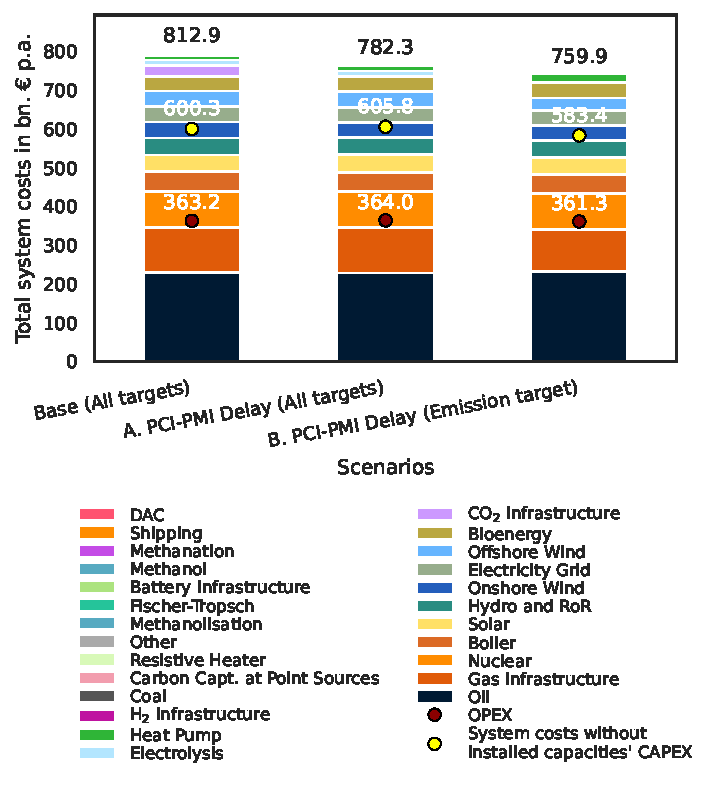
\includegraphics[width=\linewidth]{system_costs}
  \caption{Results --- Total system costs by technology and infrastructure. Own illustration.}
  \label{fig:system_costs}
\end{figure}

\subsection{Limitations of our study}
\begin{itemize}
  \item Haversine distance for level playing field
  \item No discetisation of pipelines
  \item Regional resolution for computational reasons
  \item ...
\end{itemize}

\newpage
\section{Conclusion}
\label{sec:conclusion}
We conclude that although all three EU policy targets for 2030 can be achieved without PCI-PMI infrastructure, they bring additional benefits: i) \ce{H2} pipelines projects help distribute more affordable green H$_2$ from northern and south-western Europe to high-demand regions in central Europe; ii) \ce{CO2} transport and storage projects help decarbonising the industry by connecting major industrial sites and their process emissions to offshore sequestration sites in the North Sea (Denmark, Norway, and the Netherlands). Preliminary results have further shown that most PCI-PMI projects seem to be over-dimensioned and are not cost-optimal, as very few projects show utilisation above 1000 full-load hours. However, to adequately assess the value of PCI-PMI projects, we need to assess their benefits in future target years. Further, policy targets for 2030 are not cost-effective, although needed in the long run to reach net-zero emissions by 2050.

\paragraph{Research outlook} Next steps include the implementation of remaining PCI-PMI projects, such as hybrid offshore interconnectors (energy islands), electricity storages, and \ce{CO2} shipping routes. To evaluate the long-term value of PCI-PMI projects in a sector-coupled European energy system, we will model pathway dependencies towards 2050. We will also assess the sensitivity of the infrastructure to technology-specific build-out rates.


\newpage
\section*{CRediT authorship contribution statement}
\textbf{Bobby Xiong}: Conceptualisation, Methodology, Software, Validation, Investigation, Data curation, Writing, Visualisation. \textbf{Iegor Riepin}: Conceptualisation, Methodology, Investigation, Writing, Supervision, Funding acquisition. \textbf{Tom Brown}: Investigation, Resources, Writing, Supervision, Funding acquisition.

\section*{Declaration of competing interest}
The authors declare that they have no known competing financial interests or personal relationships that could have appeared to influence the work reported in this paper.

\section*{Data and code availability}
The entire workflow, including the custom model based on PyPSA-Eur, PCI-PMI project implementation, scenario setup, postprocessing and visualisation routines can be accessed via the GitHub repository: \newline 
\href{https://github.com/bobbyxng/pcipmi-policy-targets}{https://github.com/bobbyxng/pcipmi-policy-targets}

\section*{Acknowledgements}
This work was supported by the German Federal Ministry for Economic Affairs and Climate Action (BMWK) under Grant No. 03EI4083A (RESILIENT). This project has been funded by partners of the CETPartnership (\href{https://cetpartnership.eu}{https://cetpartnership.eu}) through the Joint Call 2022. As such, this project has received funding from the European Union's Horizon Europe research and innovation programme under grant agreement no. 101069750.


%% The Appendices part is started with the command \appendix;
%% appendix sections are then done as normal sections
\newpage
\appendix
\section{Additional material}
\label{app:additional_material}

\begin{figure}[htbp]
  \centering
  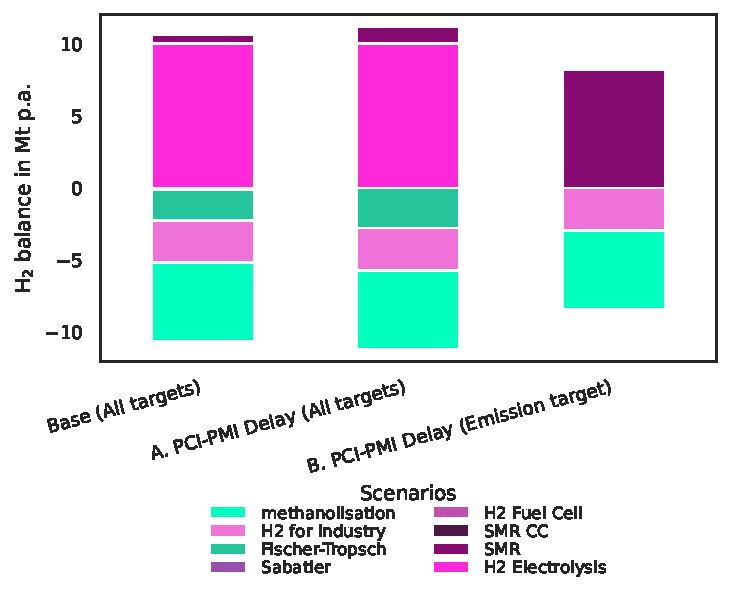
\includegraphics[width=0.9\linewidth]{h2_balance}
  \caption{Results --- \ce{H2} balance. Own illustration.}
  \label{fig:h2_balance}
\end{figure}

\begin{figure}[htbp]
  \centering
  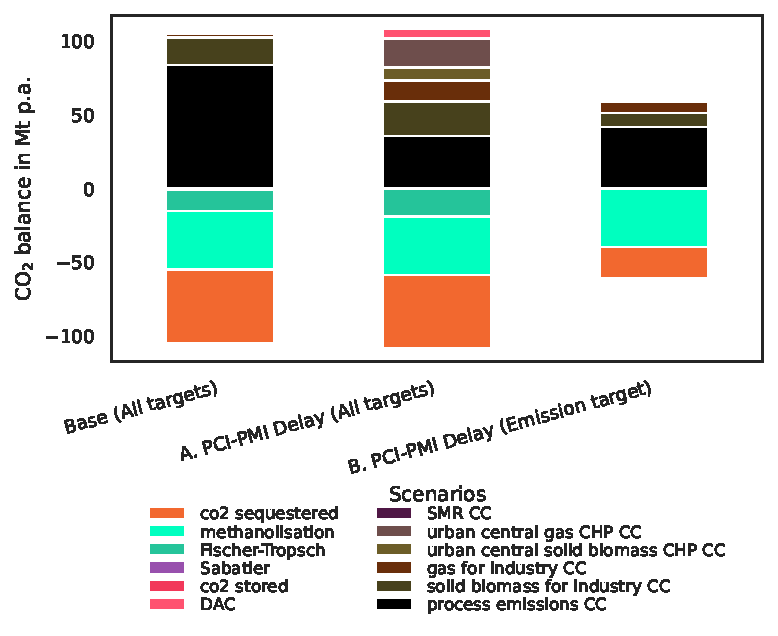
\includegraphics[width=0.9\linewidth]{co2_balance}
  \caption{Results --- \ce{CO2} balance. Own illustration.}
  \label{fig:co2_balance}
\end{figure}

\begin{figure*}[!htbp]
  \centering
  \begin{subfigure}[t]{0.47\textwidth}
      \vspace{0pt}
      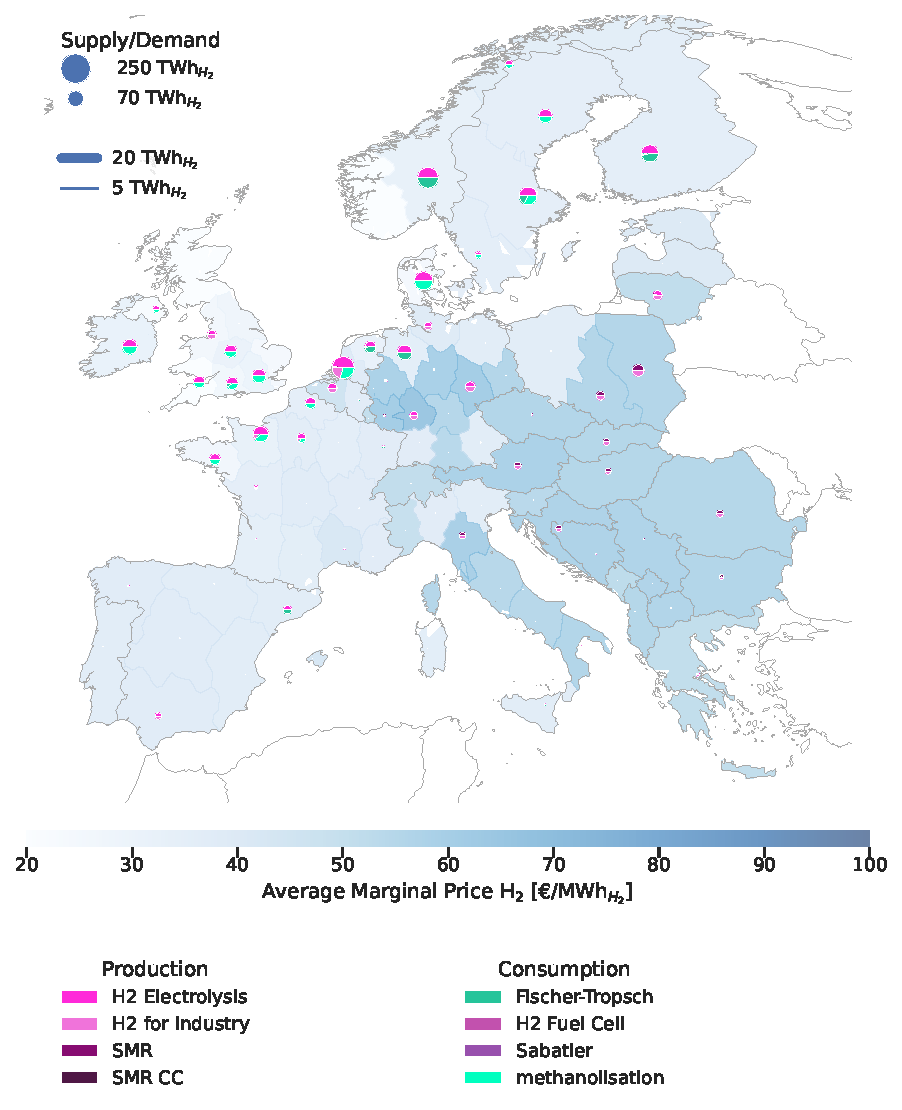
\includegraphics[width=\textwidth]{balance_map_h2_scenario_a}
      \vspace{0.3cm}
      \vspace{-0.3cm}
      \caption{\ce{H2} regional balances and flows (Scenario A, all \ce{H2} produced).}
      \label{fig:balance_map_h2_scenario_a}
  \end{subfigure}
  \hfill
  \begin{subfigure}[t]{0.47\textwidth}
      \vspace{0pt}
      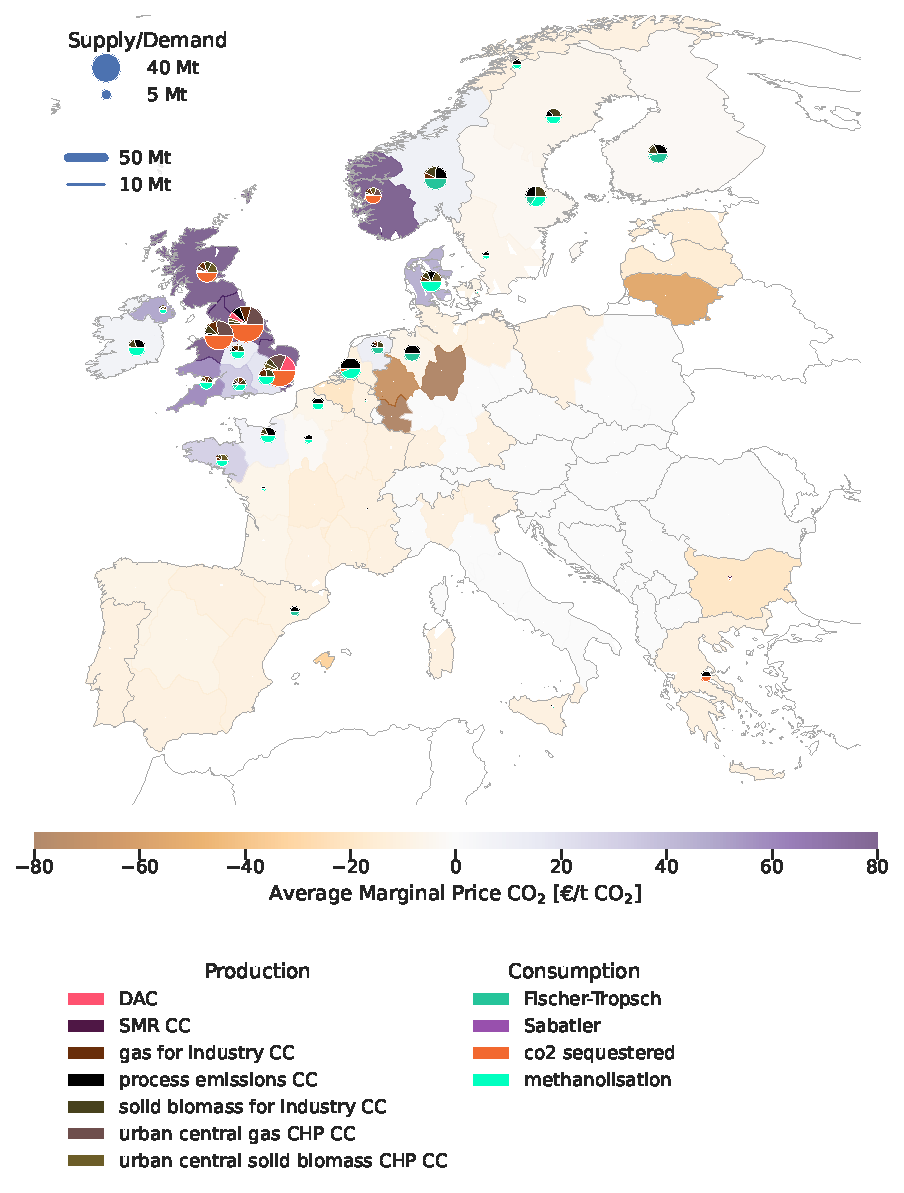
\includegraphics[width=\textwidth]{balance_map_co2_scenario_a}
      \vspace{-0.7cm}
      \caption{\ce{CO2} regional balances and flows (Scenario A).}
      \label{fig:balance_map_co2_scenario_a}
  \end{subfigure}

  \vspace{0.2cm} % Adds spacing between rows

  \begin{subfigure}[t]{0.47\textwidth}
      \vspace{0pt}
      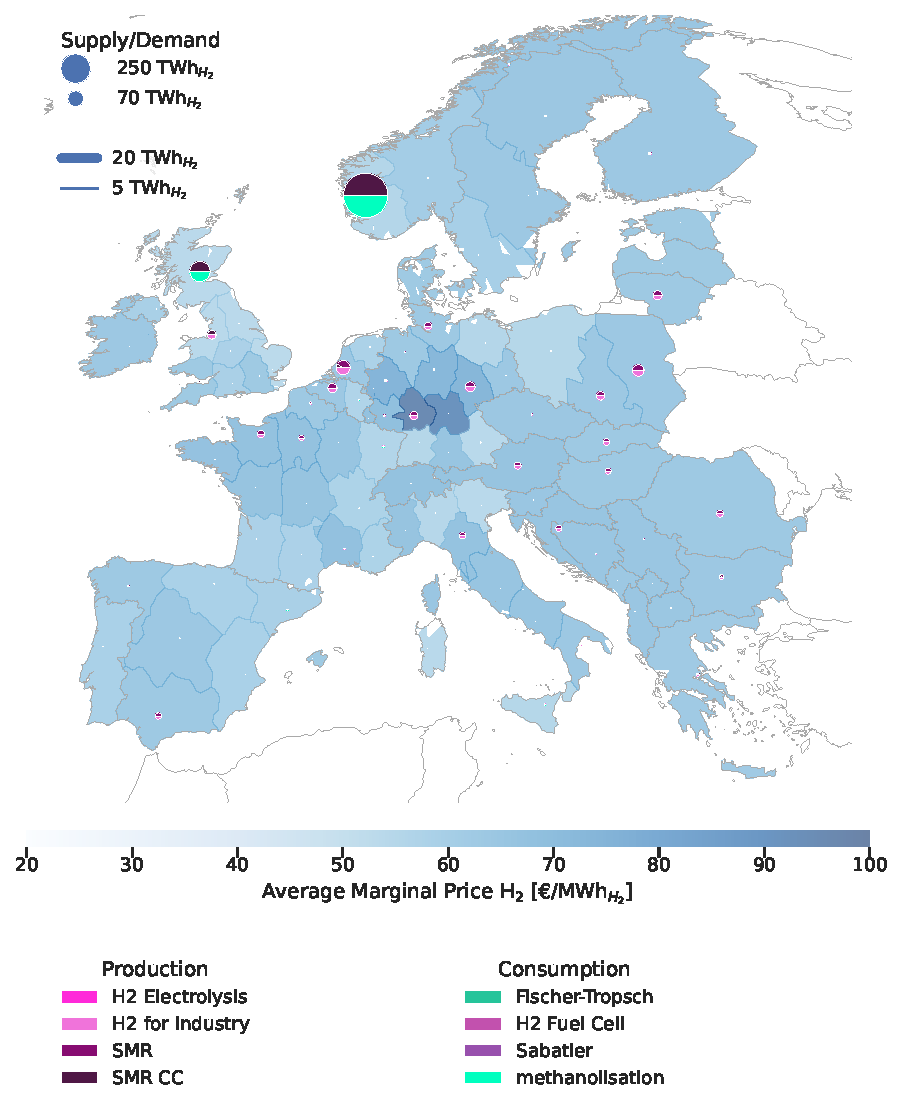
\includegraphics[width=\textwidth]{balance_map_h2_scenario_b}
      \vspace{0.3cm}
      \vspace{-0.3cm}
      \caption{\ce{H2} regional balances and flows (Scenario B, all \ce{H2} produced).}
      \label{fig:balance_map_h2_scenario_b}
  \end{subfigure}
  \hfill
  \begin{subfigure}[t]{0.47\textwidth}
      \vspace{0pt}
      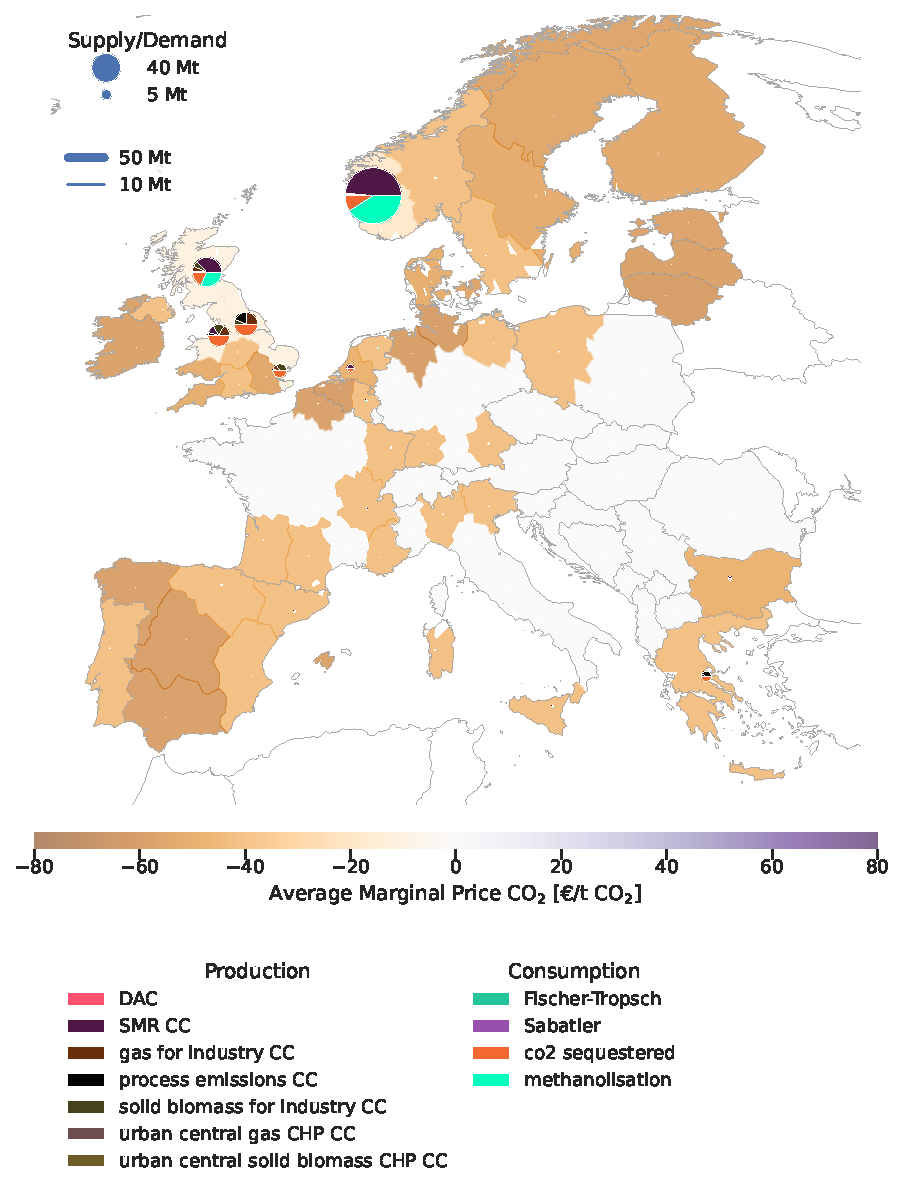
\includegraphics[width=\textwidth]{balance_map_co2_scenario_b}
      \vspace{-0.7cm}
      \caption{\ce{CO2} regional balances and flows (Scenario B).}
      \label{fig:balance_map_co2_scenario_b}
  \end{subfigure}

  \caption{Results scenarios \textit{A} and \textit{B} --- Regional distribution of \ce{H2} and \ce{CO2} production, utilisation, storage, and transport. Own illustration.}
  \label{fig:balance_maps_scenarios_a_b}
\end{figure*}

\newpage
\bibliographystyle{elsarticle-num} 
\bibliography{references.bib}

\end{document}

\endinput
%%
%% End of file `elsarticle-template-num.tex'.


%% Template related

% \section{Example Section}
% \label{sec1}
% %% Labels are used to cross-reference an item using \ref command.

% Section text. See Subsection \ref{subsec1}.

% %% Use \subsection commands to start a subsection.
% \subsection{Example Subsection}
% \label{subsec1}

% Subsection text.

% %% Use \subsubsection, \paragraph, \subparagraph commands to 
% %% start 3rd, 4th and 5th level sections.
% %% Refer following link for more details.
% %% https://en.wikibooks.org/wiki/LaTeX/Document_Structure#Sectioning_commands

% \subsubsection{Mathematics}
% %% Inline mathematics is tagged between $ symbols.
% This is an example for the symbol $\alpha$ tagged as inline mathematics.

% %% Displayed equations can be tagged using various environments. 
% %% Single line equations can be tagged using the equation environment.
% \begin{equation}
% f(x) = (x+a)(x+b)
% \end{equation}

% %% Unnumbered equations are tagged using starred versions of the environment.
% %% amsmath package needs to be loaded for the starred version of equation environment.
% \begin{equation*}
% f(x) = (x+a)(x+b)
% \end{equation*}

% %% align or eqnarray environments can be used for multi line equations.
% %% & is used to mark alignment points in equations.
% %% \\ is used to end a row in a multiline equation.
% \begin{align}
%  f(x) &= (x+a)(x+b) \\
%       &= x^2 + (a+b)x + ab
% \end{align}

% \begin{eqnarray}
%  f(x) &=& (x+a)(x+b) \nonumber\\ %% If equation numbering is not needed for a row use \nonumber.
%       &=& x^2 + (a+b)x + ab
% \end{eqnarray}

% %% Unnumbered versions of align and eqnarray
% \begin{align*}
%  f(x) &= (x+a)(x+b) \\
%       &= x^2 + (a+b)x + ab
% \end{align*}

% \begin{eqnarray*}
%  f(x)&=& (x+a)(x+b) \\
%      &=& x^2 + (a+b)x + ab
% \end{eqnarray*}

% %% Refer following link for more details.
% %% https://en.wikibooks.org/wiki/LaTeX/Mathematics
% %% https://en.wikibooks.org/wiki/LaTeX/Advanced_Mathematics

% %% Use a table environment to create tables.
% %% Refer following link for more details.
% %% https://en.wikibooks.org/wiki/LaTeX/Tables
% \begin{table}[t]%% placement specifier
% %% Use tabular environment to tag the tabular data.
% %% https://en.wikibooks.org/wiki/LaTeX/Tables#The_tabular_environment
% \centering%% For centre alignment of tabular.
% \begin{tabular}{l c r}%% Table column specifiers
% %% Tabular cells are separated by &
%   1 & 2 & 3 \\ %% A tabular row ends with \\
%   4 & 5 & 6 \\
%   7 & 8 & 9 \\
% \end{tabular}
% %% Use \caption command for table caption and label.
% \caption{Table Caption}\label{fig1}
% \end{table}


% %% Use figure environment to create figures
% %% Refer following link for more details.
% %% https://en.wikibooks.org/wiki/LaTeX/Floats,_Figures_and_Captions
% \begin{figure}[t]%% placement specifier
% %% Use \includegraphics command to insert graphic files. Place graphics files in 
% %% working directory.
% \centering%% For centre alignment of image.
% \includegraphics{example-image-a}
% %% Use \caption command for figure caption and label.
% \caption{Figure Caption}\label{fig1}
% %% https://en.wikibooks.org/wiki/LaTeX/Importing_Graphics#Importing_external_graphics
% \end{figure}

%% For citations use: 
%%       \cite{<label>} ==> [1]

%%
% Example citation, See \cite{lamport94}.

%% If you have bib database file and want bibtex to generate the
%% bibitems, please use

%% else use the following coding to input the bibitems directly in the
%% TeX file.

%% Refer following link for more details about bibliography and citations.
%% https://en.wikibooks.org/wiki/LaTeX/Bibliography_Management

% \begin{thebibliography}{00}

% %% For numbered reference style
% %% \bibitem{label}
% %% Text of bibliographic item

% \bibitem{lamport94}
%   Leslie Lamport,
%   \textit{\LaTeX: a document preparation system},
%   Addison Wesley, Massachusetts,
%   2nd edition,
%   1994.

% \end{thebibliography}